%!TEX root = ../main.tex

\section{Implementation Details of Baselines}
\label{sec:appendix_baselines}

In this section, we provide the implementation details of all baselines compared in our experiments, including their prompt templates, configuration choices, and the comparison with agentic coding systems.

\subsection{Prompt Templates of Baselines}
\label{subsec:prompts_of_baselines}

We present the prompt templates used by each baseline. All methods share the same prompt structure consisting of \texttt{Role}, \texttt{Demonstration}, and \texttt{Hint} sections. For operator-assisted methods, an additional \texttt{Operator Space} section is included. All methods use the same ADP demonstration cases for In-Context Learning. We omit the operator definition and demonstration examples in the prompt figures due to the space limit.

\begin{figure}[!t]
    \centering 
    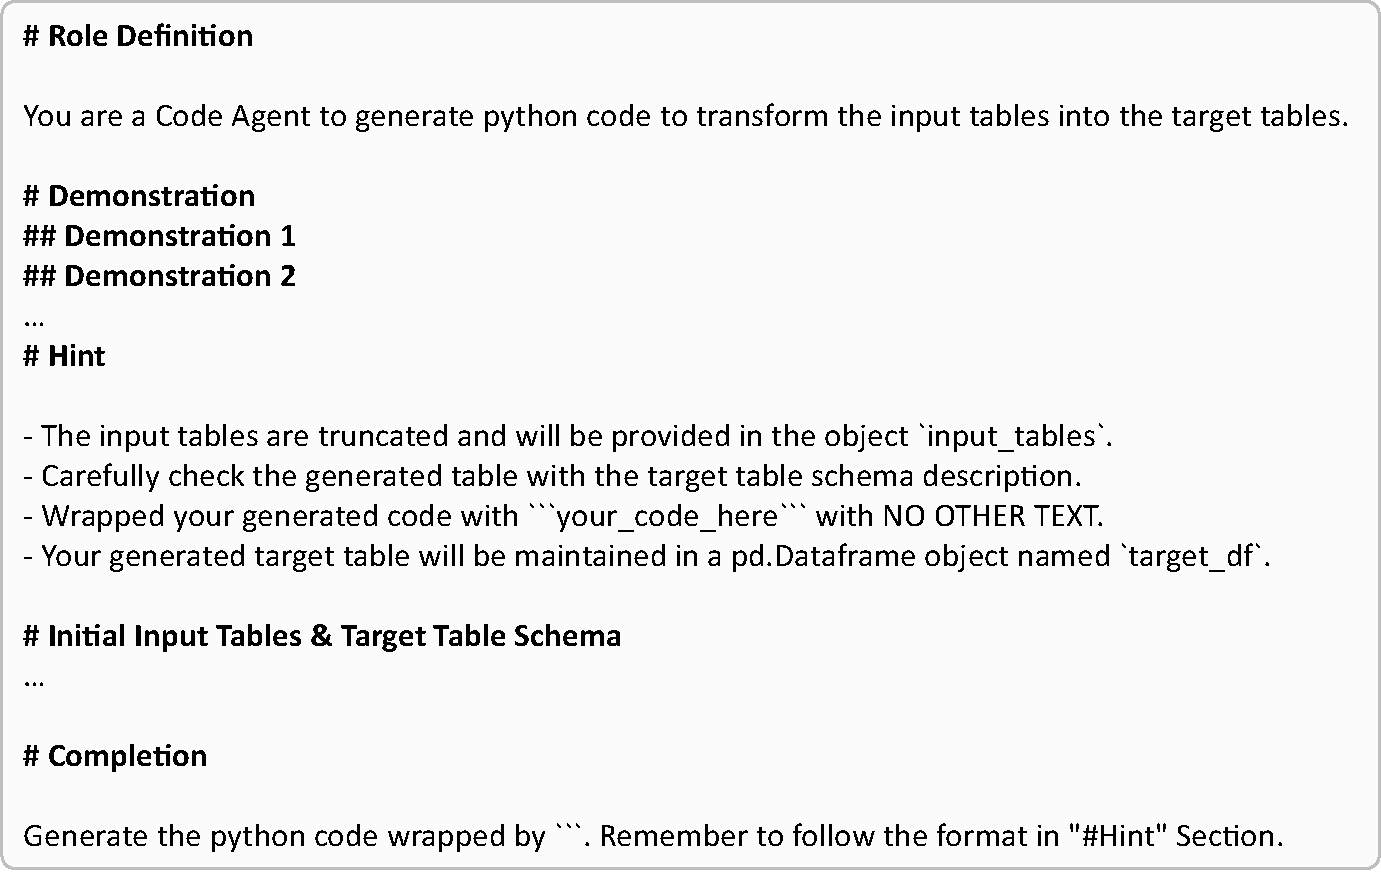
\includegraphics[width=0.99\columnwidth]{appendix/figures/fig/code_gen_prompt.pdf}
    \vspace{-1em}
    \caption{Prompt of CodeGen.
    }
    \label{fig:code_gen_prompt}
    % \vspace{-1em}
\end{figure}

\begin{figure}[!t]
    \centering 
    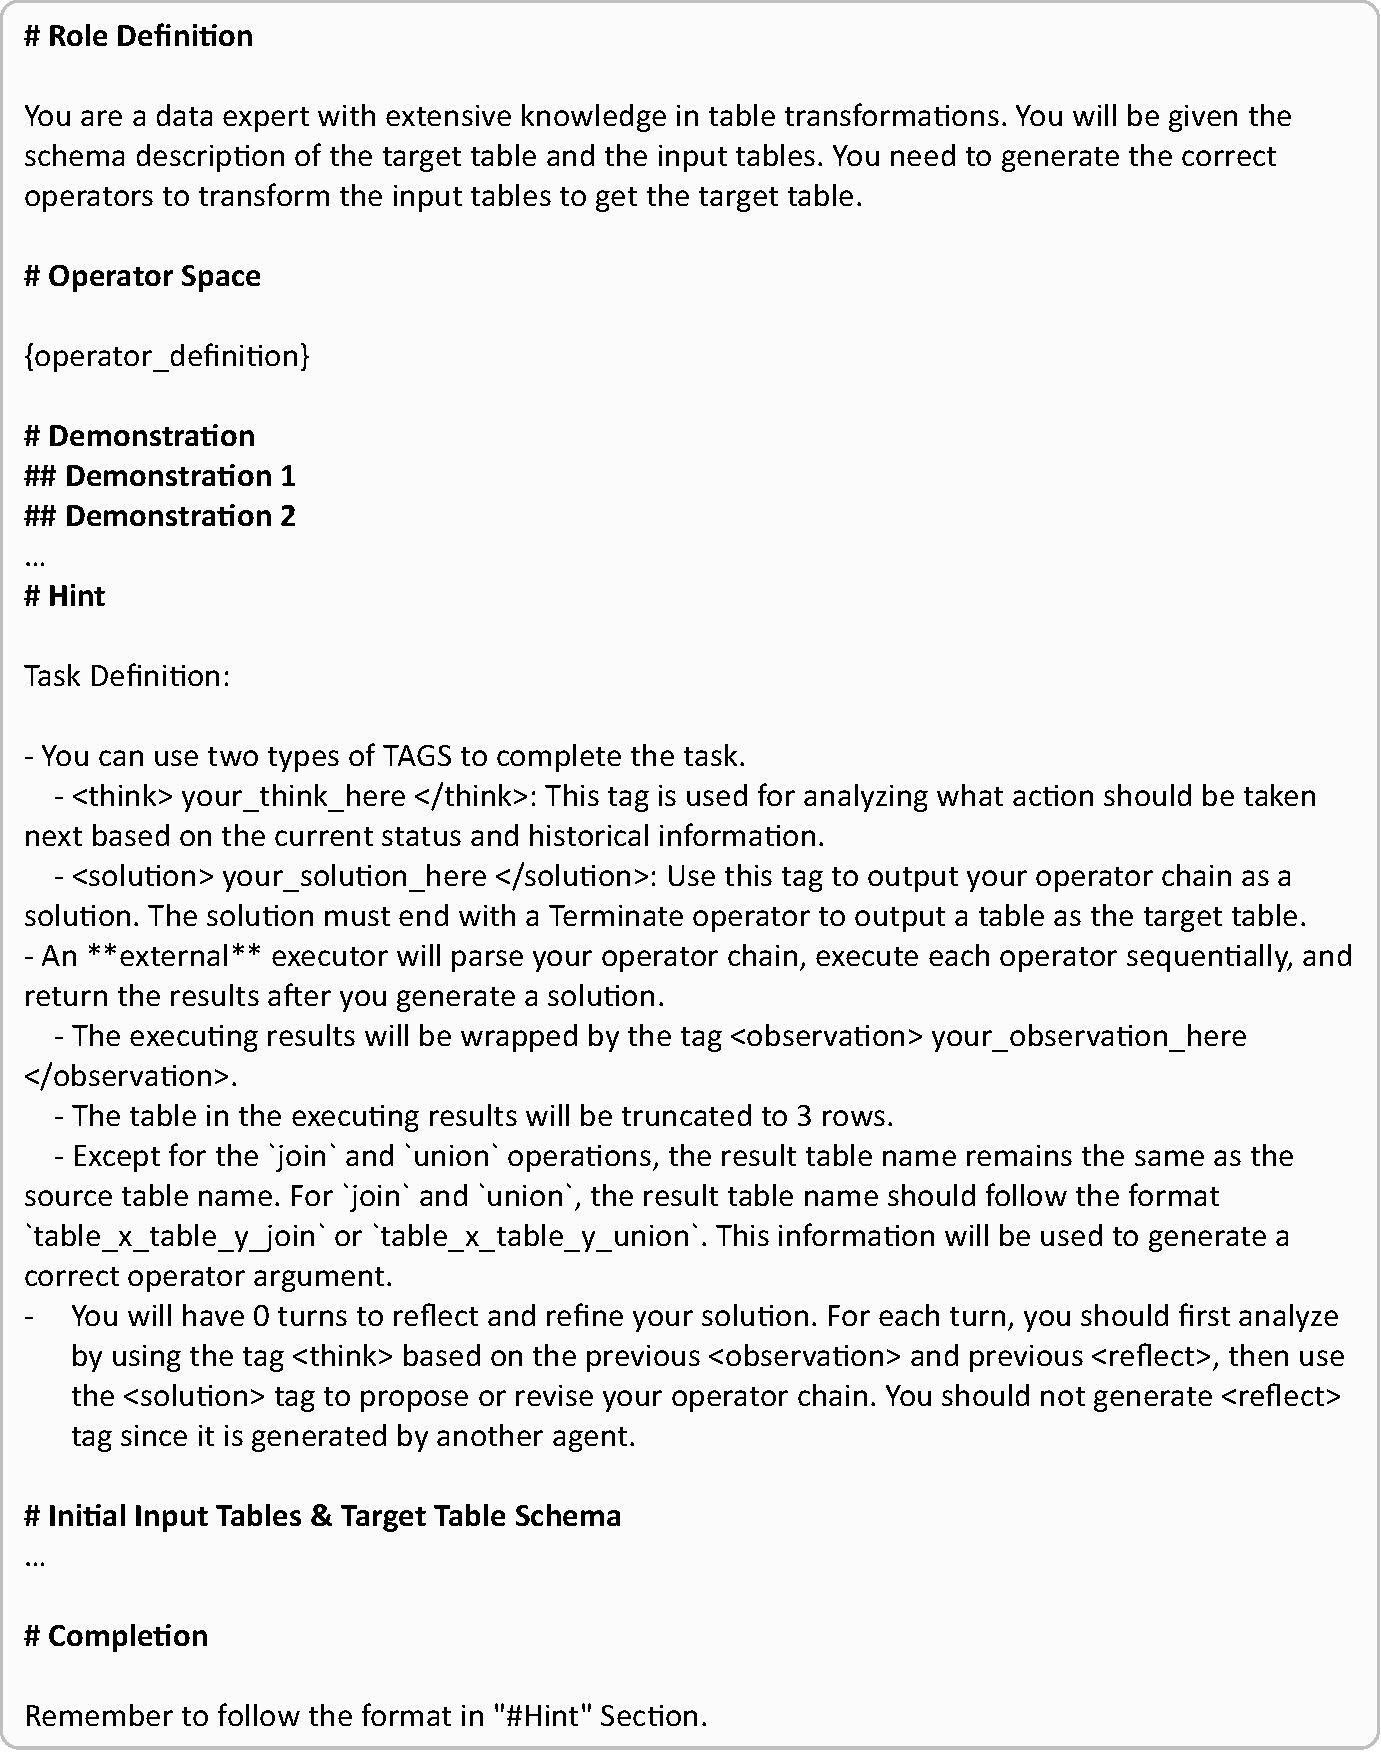
\includegraphics[width=0.99\columnwidth]{appendix/figures/fig/planandaction_prompt.pdf}
    \vspace{-1em}
    \caption{Prompt of PlanAndAction.
    }
    \label{fig:planandaction_prompt}
    % \vspace{-1em}
\end{figure}

\begin{figure}[!t]
    \centering 
    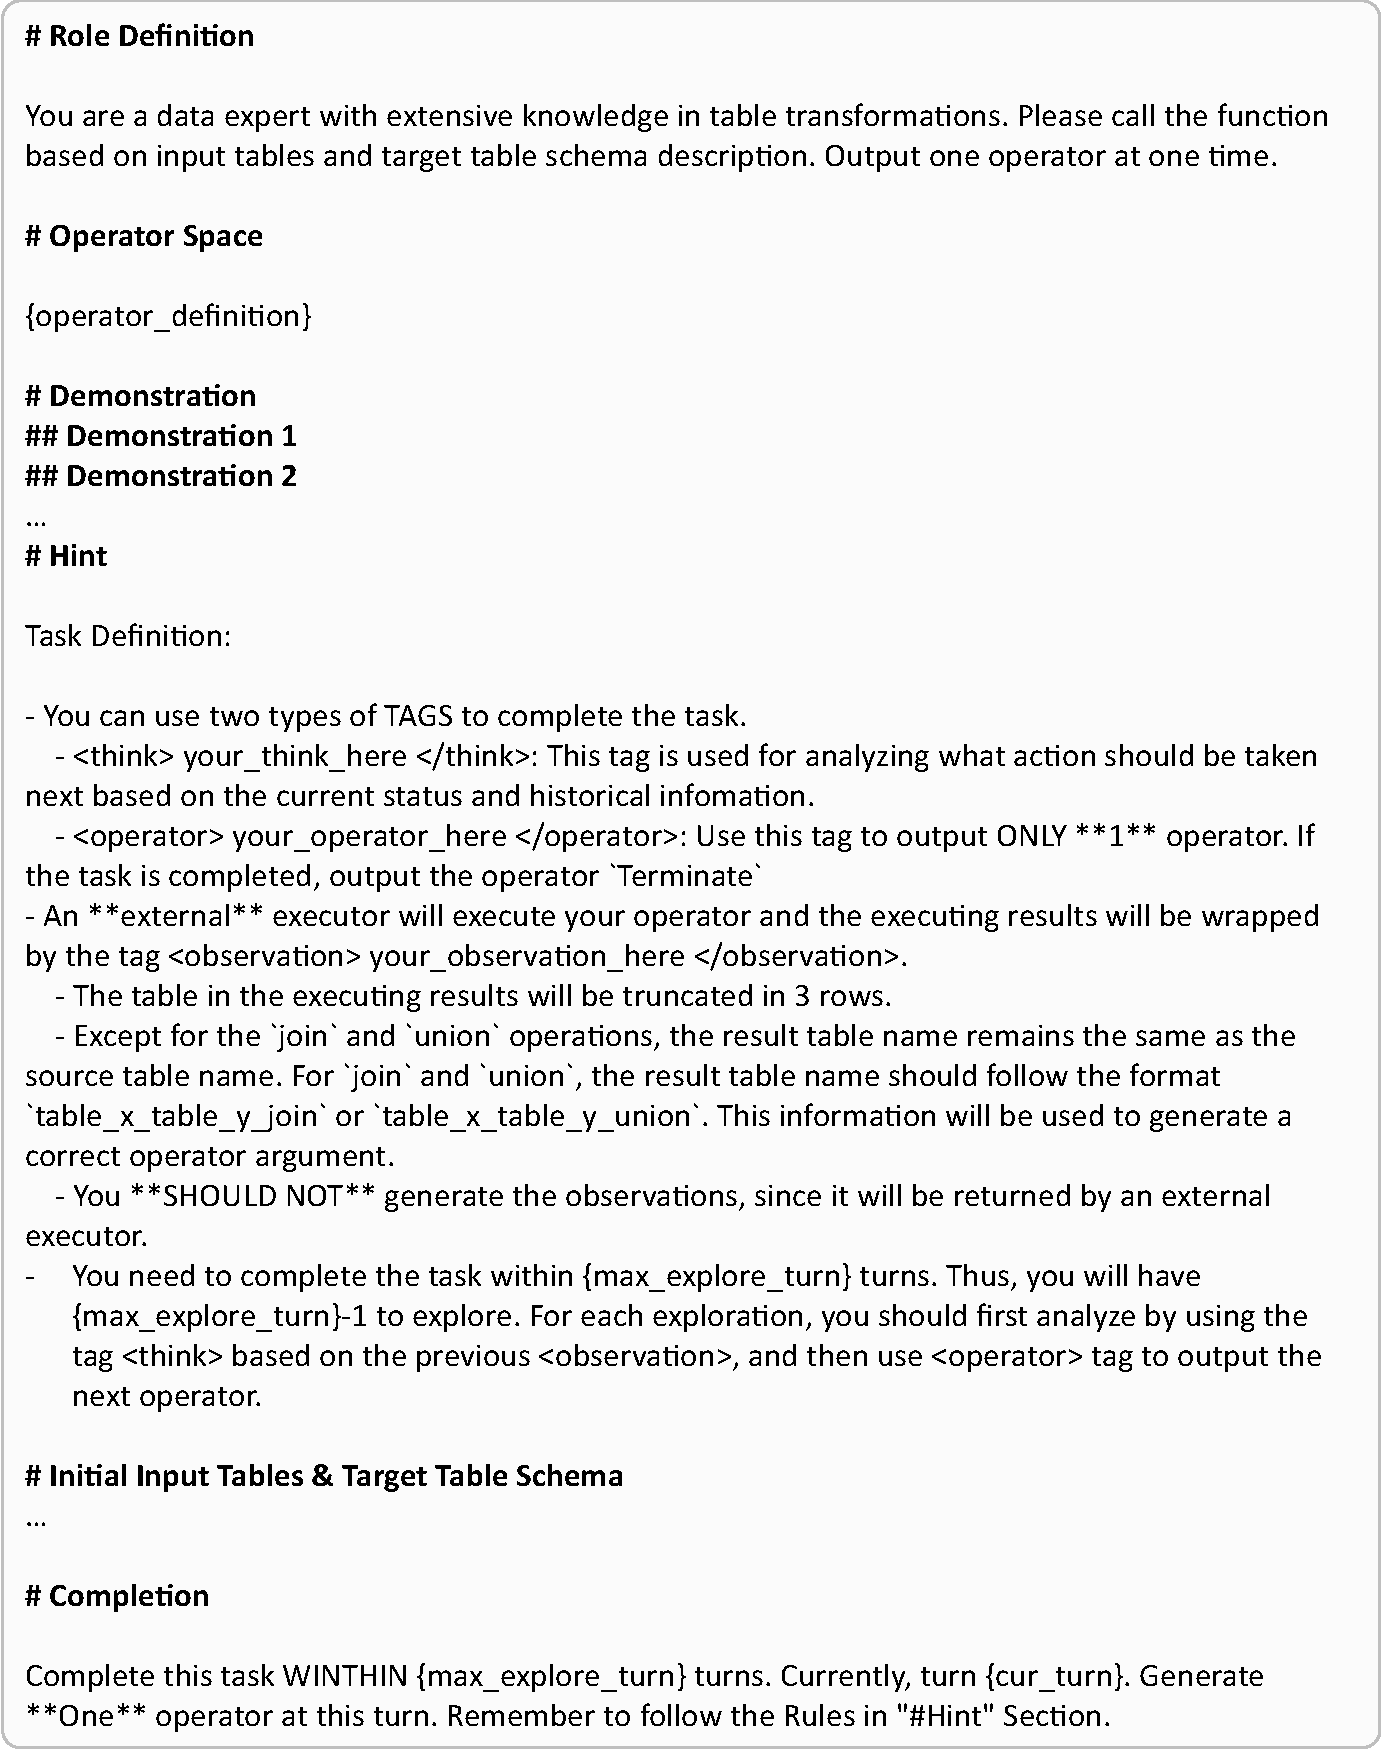
\includegraphics[width=0.99\columnwidth]{appendix/figures/fig/react_prompt.pdf}
    \vspace{-1em}
    \caption{Prompt of ReAct.
    }
    \label{fig:react_prompt}
    % \vspace{-1em}
\end{figure}

\begin{figure}[!t]
    \centering 
    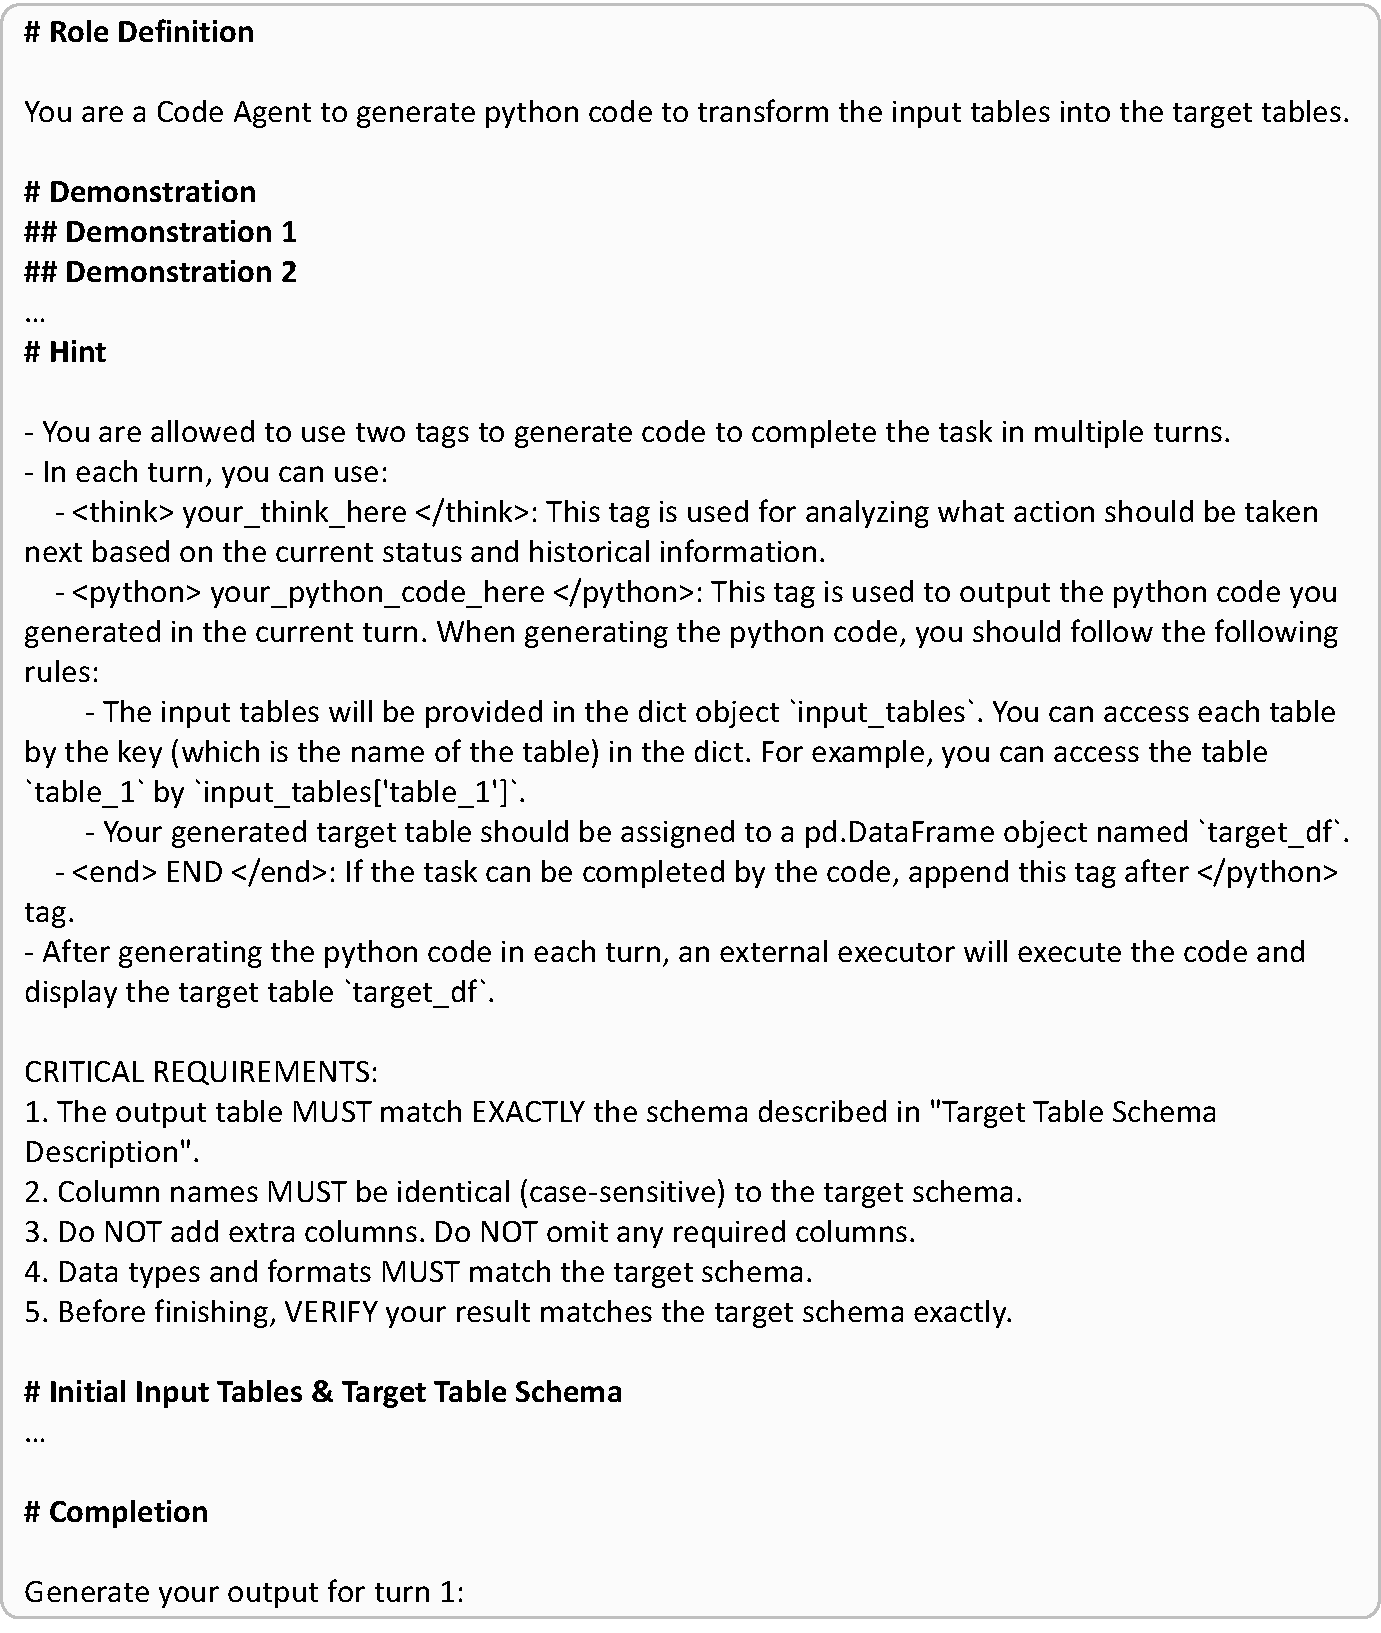
\includegraphics[width=1.01\columnwidth]{appendix/figures/fig/code_agent_prompt.pdf}
    \vspace{-2em}
    \caption{Prompt of CodeGen baseline.
    }
    \label{fig:code_agent_prompt}
\end{figure}

\begin{figure}[!t]
    \centering 
    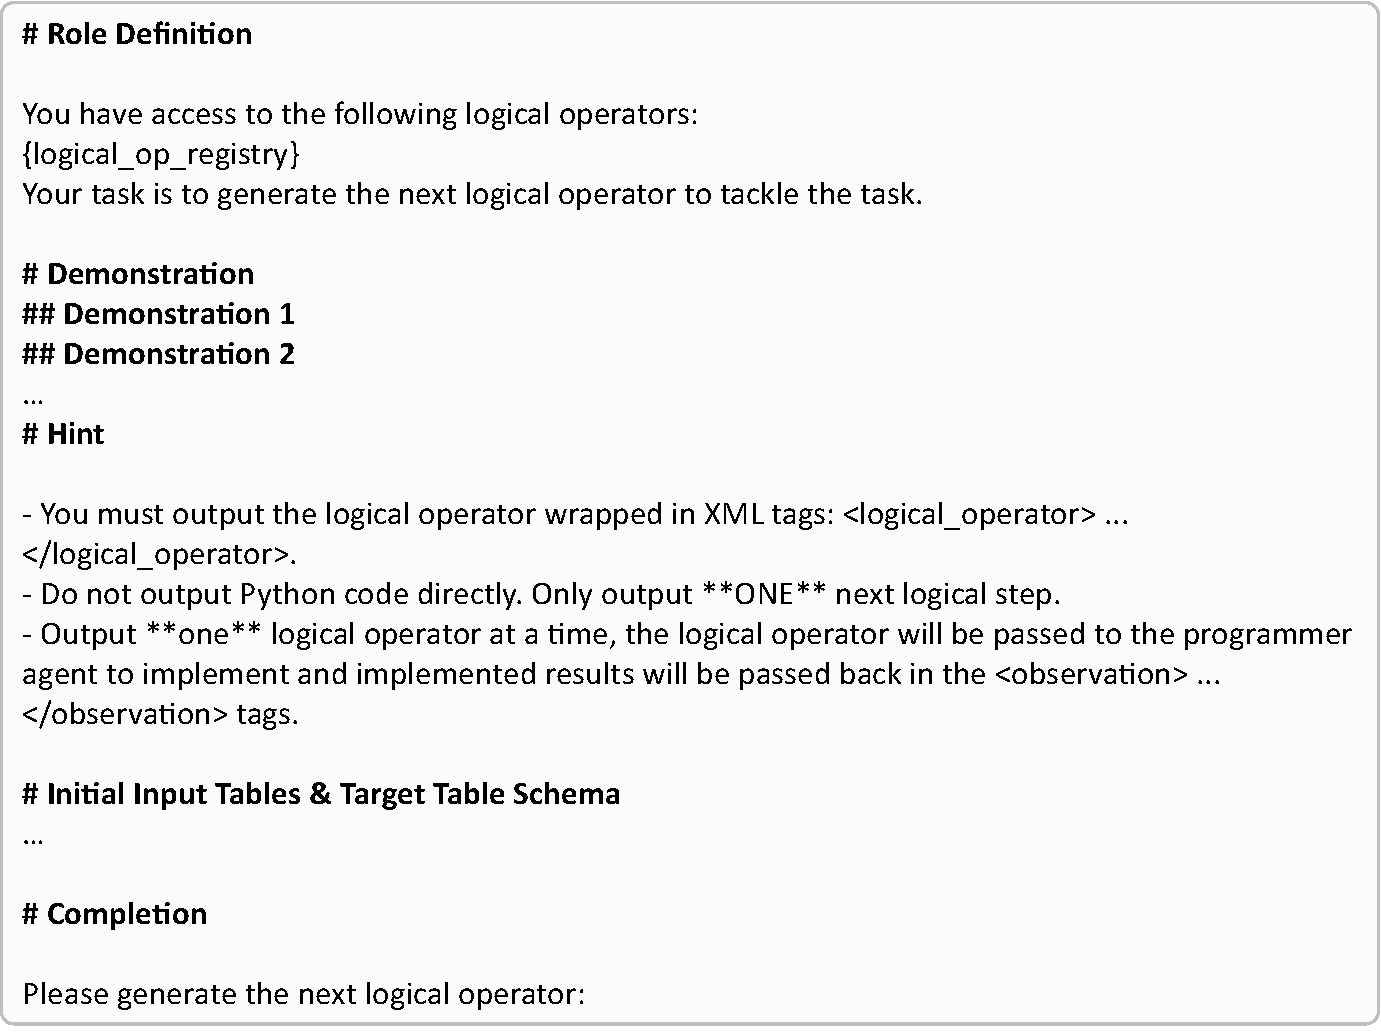
\includegraphics[width=0.99\columnwidth]{appendix/figures/fig/autoprep_planner_prompt.pdf}
    \vspace{-1em}
    \caption{Prompt of AutoPrep Planner.
    }
    \label{fig:autoprep_planner_prompt}
    % \vspace{-1em}
\end{figure}

\begin{figure}[!t]
    \centering 
    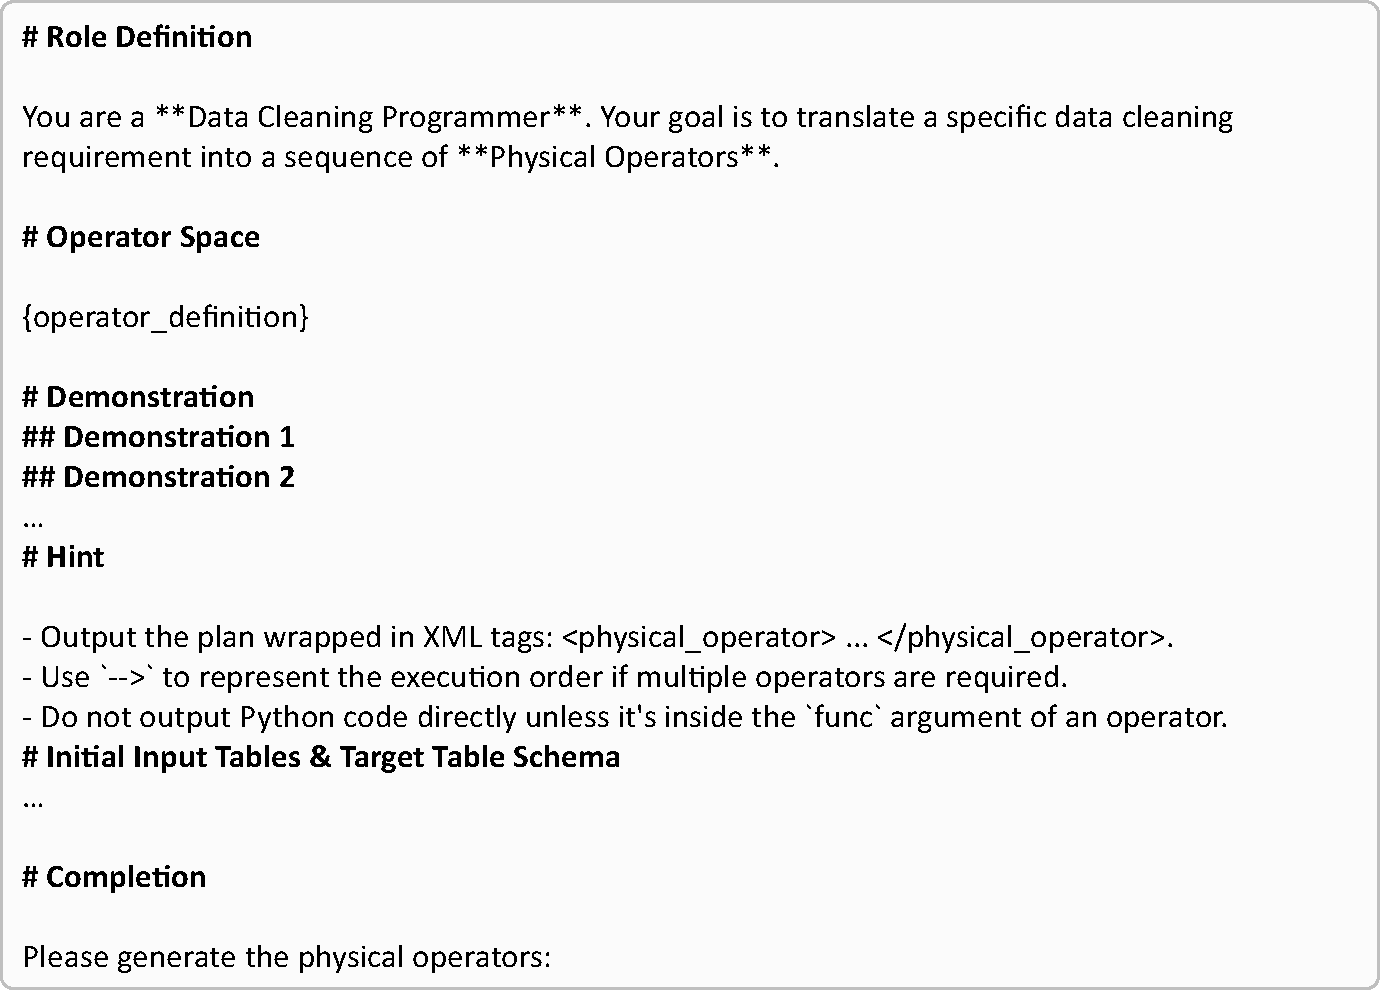
\includegraphics[width=0.99\columnwidth]{appendix/figures/fig/autoprep_programmer_prompt.pdf}
    \vspace{-1em}
    \caption{Prompt of AutoPrep Programmer.
    }
    \label{fig:autoprep_programmer_prompt}
    % \vspace{-1em}
\end{figure}

\begin{figure}[!t]
    \centering 
    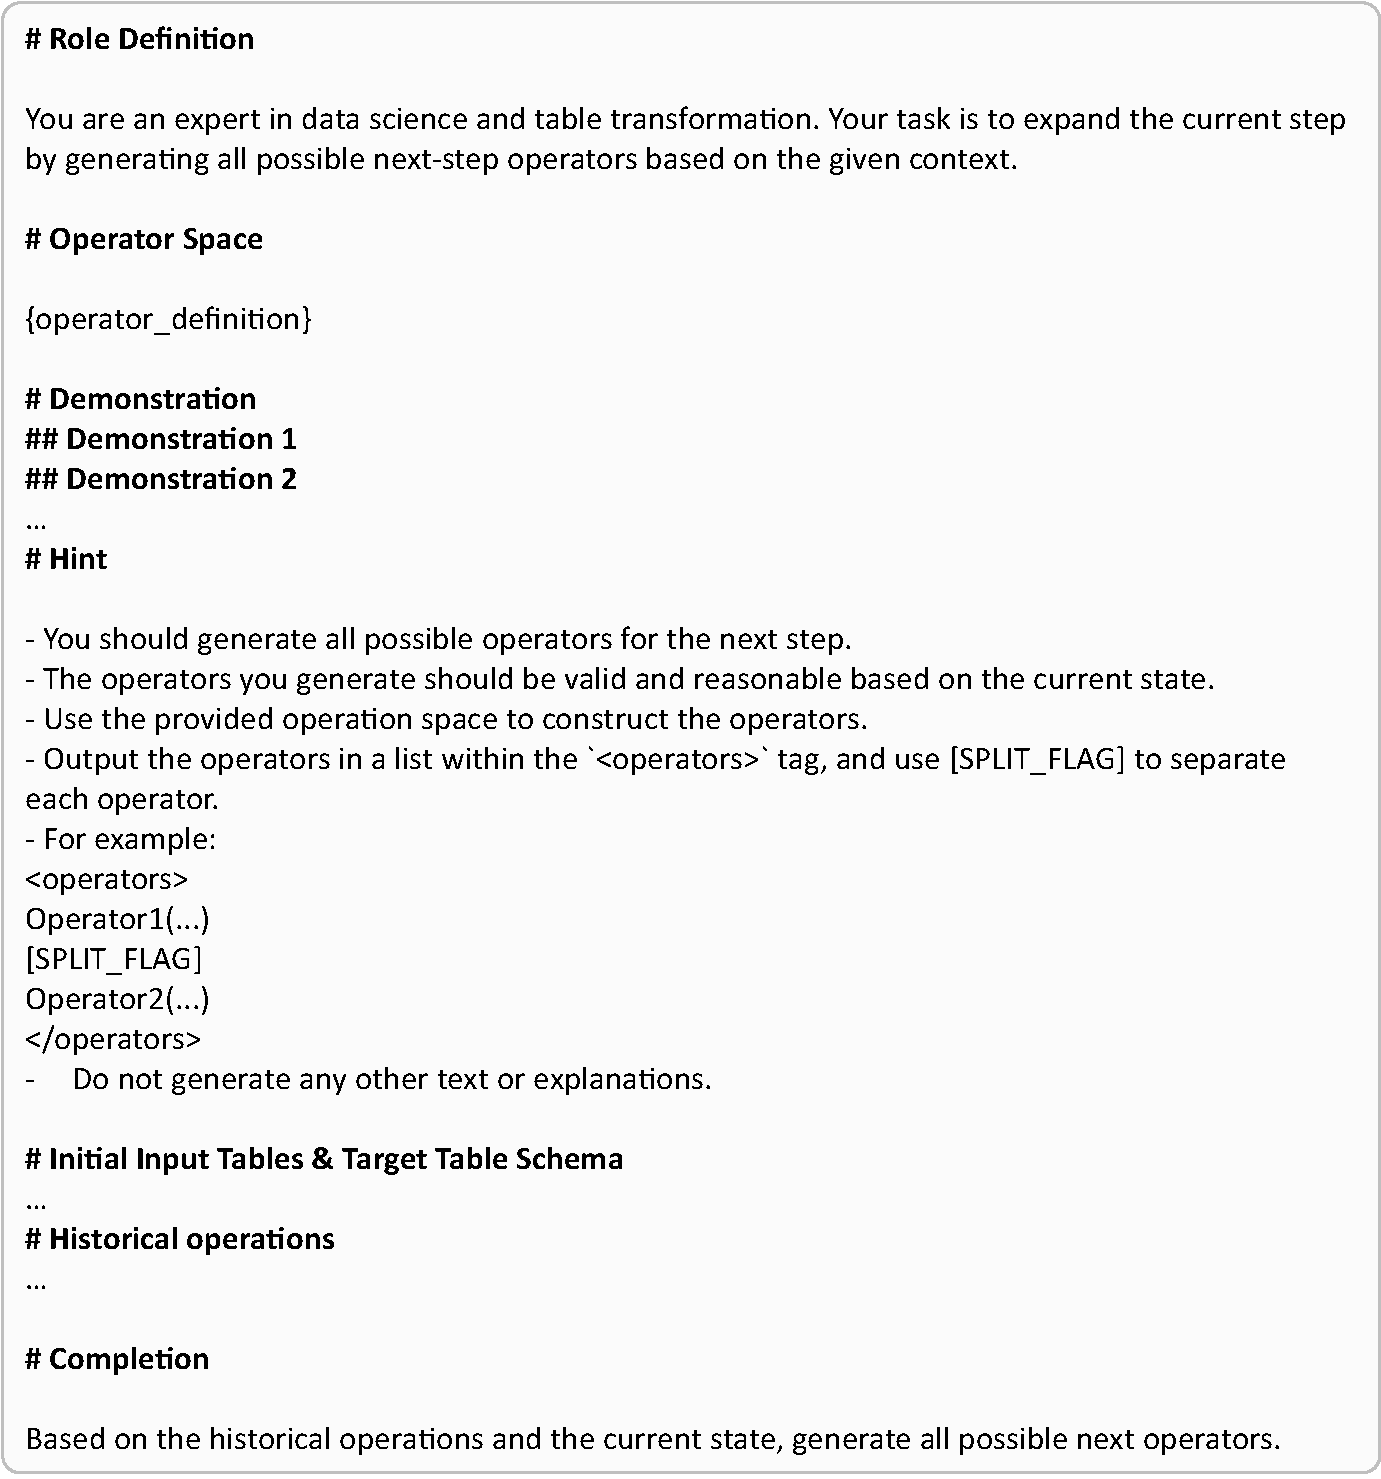
\includegraphics[width=0.99\columnwidth]{appendix/figures/fig/mcts_expand_prompt.pdf}
    \vspace{-1em}
    \caption{Prompt of MCTS-OP Expand.
    }
    \label{fig:mcts_expand_prompt}
    % \vspace{-1em}
\end{figure}

\begin{figure}[!t]
    \centering 
    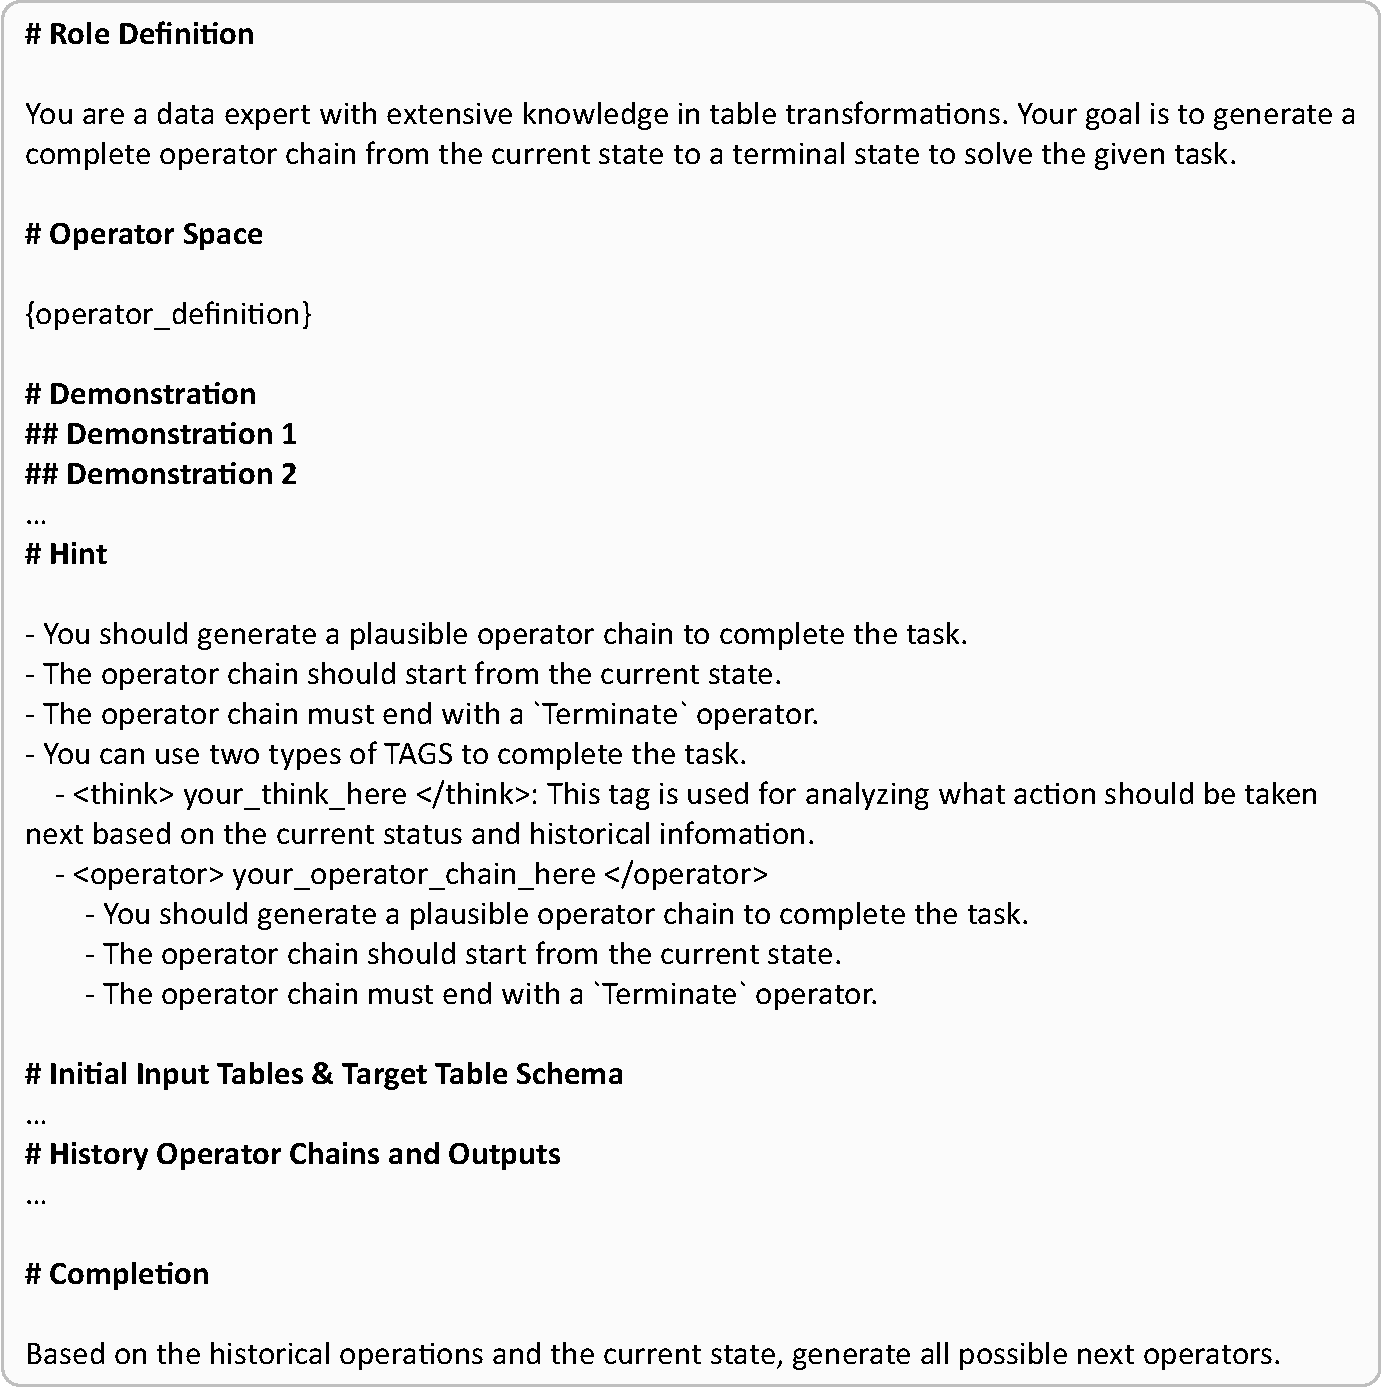
\includegraphics[width=0.99\columnwidth]{appendix/figures/fig/mcts_simulation_prompt.pdf}
    \vspace{-1em}
    \caption{Prompt of MCTS-OP Simulation.
    }
    \label{fig:mcts_simulation_prompt}
    % \vspace{-1em}
\end{figure}

\begin{figure}[!t]
    \centering 
    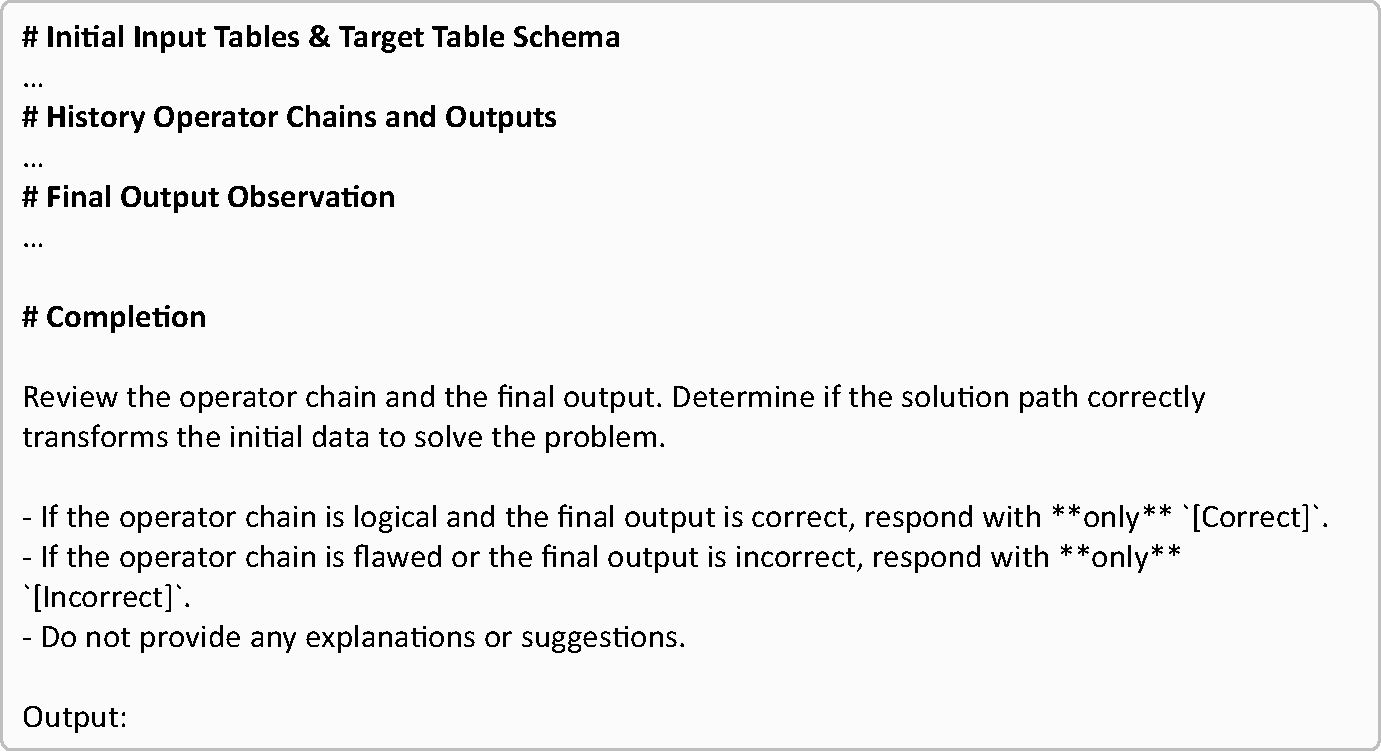
\includegraphics[width=0.99\columnwidth]{appendix/figures/fig/mcts_reward_prompt.pdf}
    \vspace{-1em}
    \caption{Prompt of MCTS-OP Reward.
    }
    \label{fig:mcts_reward_prompt}
    % \vspace{-1em}
\end{figure}


\stitle{CodeGen.}
As shown in Figure~\ref{fig:code_gen_prompt}, this method treats the data preparation task as a standard programming problem.
The prompt defines the model's role as a Code Agent, responsible for generating Python code to transform source tables into a target table. To ensure the generated code is executable and evaluable, the prompt imposes strict formatting constraints in the ``Hint'' section. Specifically, the model is required to wrap the code within triple backticks and ensure the final result is stored in a specific \texttt{pd.DataFrame} object named \texttt{target\_df}.
At each turn, the execution result of the generated Python code is appended to the prompt, serving as a signal to revise the code at the next turn. The agent iterates until exceeding the maximum turn or actively ending the task with an \action{end} tag.

\stitle{Plan-and-Solve (PaS).}
As shown in Figure~\ref{fig:planandaction_prompt}, this method restricts the model to a predefined set of operator types to improve controllability.
The prompt defines the model as a ``data expert'' and provides a specific \texttt{operator\_definition} space.
To facilitate reasoning and interaction with the environment, the prompt instructs the model to use specific XML tags:
(1) \action{think}: Used for analyzing the current execution state and planning the next step;
(2) \action{solution}: Used to output the operator sequence for the current step;
(3) \action{observation}: A placeholder for the execution feedback returned by the environment.
Furthermore, the prompt specifies naming conventions for intermediate tables (especially for \texttt{Join} and \texttt{Union} operations) to ensure the operator parameters remain consistent across steps.

\stitle{ReAct.}
As illustrated in Figure~\ref{fig:react_prompt}, this method adopts a linear ReAct-style interaction loop to solve the task.
The prompt limits the model to generate exactly one operator instance per turn using the \action{operator} tag, preceded by a specific analysis step using the \action{think} tag.
Unlike the single-pass methods, ReAct is explicitly aware of a maximum exploration turns limit (\texttt{max\_explore\_turn}), encouraging it to dynamically adjust its subsequent decisions based on the execution feedback (\action{observation}) returned by the environment.
Similar to Plan-and-Solve, it also enforces strict naming conventions for \texttt{Join} and \texttt{Union} operations to maintain context across the multi-turn interaction.

\stitle{DeepAnalyze.}
Figure~\ref{fig:code_agent_prompt} presents the prompt for the DeepAnalyze baseline.
In contrast to the standard CodeGen method, this approach allows the model to interact with the environment over multiple turns.
The prompt instructs the model to use \action{think} for analyzing the current execution state and \action{python} to output data processing programs for the current turn.
Crucially, the prompt includes a ``CRITICAL REQUIREMENTS'' section, which explicitly emphasizes strict schema alignment (\eg case-sensitive column names, exact data types) to guide the model in self-correction before finalizing the task with the \action{end} tag.

\stitle{AutoPrep.}
We implement AutoPrep using a hierarchical multi-agent framework, consisting of a Planner and several Programmers.
(1) \textbf{AutoPrep Planner.} As shown in Figure~\ref{fig:autoprep_planner_prompt}, the Planner operates at a high level. It is provided with a registry of logical operators (\action{logical\_op\_registry}) and is tasked with generating the next abstract logical plan (\eg ``clean data'') wrapped in \action{logical\_operator} tags. It does not write code or specify operator parameters.
(2) \textbf{AutoPrep Programmer.} As shown in Figure~\ref{fig:autoprep_programmer_prompt}, the Programmer receives the logical plan and translates it into a data preparation pipeline of executable operators. It has access to the full set of supported data preparation operators and uses the \texttt{-->} symbol to represent the application order of multiple operators (\eg \texttt{SplitColumn --> RenameColumn}) required to fulfill a single logical intent.
Since AutoPrep was originally designed for TableQA rather than autonomous data preparation, we replace its original prompt with an ADP-oriented prompt and apply the same tuning procedure as \sys.

\stitle{MCTS-OP.}
We implement a Monte Carlo Tree Search (MCTS) baseline adapted for operator generation. This method decomposes the reasoning process into three distinct phases, each governed by a specific prompt:

(1) \textbf{Expansion:} As shown in Figure~\ref{fig:mcts_expand_prompt}, this prompt is used to grow the search tree. The model is instructed to analyze the current history and generate a list of ``all possible next-step operators'' that are valid and reasonable. To facilitate parsing by the search algorithm, the model must output each candidate operator in a structured format within \action{op\_i} tags, where $i$ is the candidate index.

(2) \textbf{Simulation (Rollout):} As shown in Figure~\ref{fig:mcts_simulation_prompt}, this prompt is used to estimate the value of a node by completing a partial pipeline. Given the current operator history, the model generates a continuation of the operator chain that leads to the target table. The prompt instructs the model to output the remaining operators within a \texttt{<completion>} tag.

(3) \textbf{Reward:} As shown in Figure~\ref{fig:mcts_reward_prompt}, this prompt evaluates the quality of a completed pipeline. The model is asked to assess the generated operator chain by comparing the resulting table with the target schema description. It outputs a numerical score within a \action{score} tag, which is used as the node value for backpropagation in the MCTS algorithm.

\stitle{MontePrep.}
MontePrep~\cite{ge2025monteprep} applies Monte Carlo Tree Search and performs tree search over actions such as schema mapping, operator discovery, code synthesis, and refinement instead of individual operators. We use the authors' released code with default settings.

\stitle{TRAE.}
TRAE is an open-source agentic coding system developed by ByteDance\footnote{\url{https://github.com/bytedance/trae-agent}}, which has shown strong performance on SWE-bench~\cite{jimenez2024swe}. We evaluate it as a representative of state-of-the-art agentic coding systems.

\stitle{Claude Code (CC).}
Claude Code is a commercial AI-powered IDE that integrates agentic coding capabilities with planning, code generation, execution, and iterative refinement loops. We install Claude Code v2.1.119 and evaluate it using the Claude-4 backbone, as required by its framework.

\subsection{Configuration and Tuning Details}
\label{subsec:appendix_baseline_config}

To ensure fair and reproducible comparisons, we apply a consistent configuration and tuning methodology across all baselines.

\stitle{Methods with Publicly Available Implementations.}
For methods with publicly available implementations, including MontePrep~\cite{ge2025monteprep}, DeepAnalyze~\cite{zhang2025deepanalyze}, AutoPrep~\cite{fan2024autoprep}, and MCTS-OP~\cite{li2025alphasql}, we use their official codebases and default configurations (\eg prompt design, parameters, etc.).

\stitle{Methods Requiring Reimplementation.}
For methods without publicly available implementations, including CodeGen, ReAct, and PaS, we reimplemented them following the descriptions in their papers and applied the same prompt-tuning and parameter-selection procedure used for \sys. Therefore, all methods were evaluated under a comparable tuning method.

\stitle{Methods Requiring Adaptation.}
When a method was originally designed for a different task and could not be directly applied to ADP, we adapted its prompt to the ADP setting and tuned its parameters using the same grid-search procedure adopted by \sys. For example, AutoPrep was originally designed for TableQA rather than autonomous data preparation, so we replaced its original prompt with an ADP-oriented prompt and tuned it accordingly.

\stitle{Shared Configuration.}
All methods share the following configuration:
\begin{itemize}[leftmargin=*]
    \item \textbf{Prompt structure.} All methods share the same prompt structure consisting of \texttt{Role}, \texttt{Demonstration}, and \texttt{Hint} sections. For operator-assisted methods, an additional \texttt{Operator Space} section is included.
    \item \textbf{Demonstration.} All methods use the same ADP demonstration cases for In-Context Learning.
    \item \textbf{Serialization.} All methods share the same serialization function and hyperparameters (maximum column number and row number) for table serialization.
    \item \textbf{Temperature.} For all prompting methods, the temperature is set to 0.01 to ensure reproducibility.
    \item \textbf{Maximum exploration turns.} The maximum exploration turn is set to 5 for methods that require specifying this hyperparameter, including \sys, CodeGen, and DeepAnalyze.
    \item \textbf{Training baselines.} Training baselines (IL, RL-GRPO) use the same backbone models and hyperparameters as \sys, differing only in the training strategy. This isolates the effect of our progressive agentic training.
\end{itemize}

\subsection{Comparison with Agentic Coding Systems}
\label{subsec:appendix_agentic_coding}

Following the suggestion of Reviewer~\#1, we compare \sys with two strong agentic coding systems: Claude Code (CC) and TRAE. These systems represent state-of-the-art general-purpose coding agents that implement planning--coding--testing loops with environment feedback.

\begin{table}[t]
  \centering
  \caption{\bf Comparison between \sys and Agentic Coding Systems.}
  \vspace{-1em}
  \label{\labelprefix tbl:agentic_coding_system_exp}
  \resizebox{0.98\columnwidth}{!}{
    \begin{tabular}{|c|c||c|c|c|c|c|c|}
      \hline
      \multirow{2}{*}{\textbf{LLM}} & \multirow{2}{*}{\textbf{Method}} 
      & \multicolumn{2}{c|}{\textbf{Synth-Spider}} 
      & \multicolumn{2}{c|}{\textbf{Synth-Bird}} 
      & \multicolumn{2}{c|}{\textbf{Parrot}} \\
      \cline{3-8}
      & & \textbf{Acc.} & \textbf{Cost (\$)} 
        & \textbf{Acc.} & \textbf{Cost (\$)} 
        & \textbf{Acc.} & \textbf{Cost (\$)} \\
      \hline \hline

      \multirow{2}{*}{GPT-5}
        & TRAE
        & \textbf{72.36} & 0.038
        & \textbf{61.75} & 0.033
        & 41.19 & 0.041 \\
        \cline{2-8}

        & \textbf{\sys}
        & 71.76 & \textbf{0.014}
        & 60.46 & \textbf{0.015}
        & \textbf{41.33} & \textbf{0.009} \\
      \hline
      \hline

      \multirow{3}{*}{Claude-4}
        & CC
        & 72.71 & 0.169
        & \textbf{68.33} & \underline{0.141}
        & \underline{42.98} & 0.188 \\
        \cline{2-8}

        & TRAE
        & \textbf{73.80} & \underline{0.148}
        & 66.93 & 0.160
        & 41.93 & \underline{0.125} \\
        \cline{2-8}

        & \textbf{\sys}
        & \underline{73.46} & \textbf{0.054}
        & \underline{67.43} & \textbf{0.062}
        & \textbf{46.07} & \textbf{0.044} \\
      \hline
    \end{tabular}
  }
  \vspace{-1em}
\end{table}


Table~\ref{\labelprefix tbl:agentic_coding_system_exp} reports the comparison results. \sys achieves accuracy comparable to CC and TRAE across all benchmarks while \emph{consistently reducing cost}. With GPT-5, \sys achieves accuracy comparable to TRAE while reducing cost by 2.7$\times$ on Synth-Spider, 2.2$\times$ on Synth-Bird, and 4.6$\times$ on Parrot. With Claude-4, \sys achieves accuracy comparable to both CC and TRAE, while achieving the best accuracy on Parrot and reducing cost by 2.7$\times$--4.3$\times$.

\stitle{Why \sys is More Cost-Effective.}
The cost advantage of \sys over general-purpose coding agents stems from two aspects:

\begin{itemize}[leftmargin=*]
    \item \textbf{Clearer intermediate evaluation.} Since each operator produces a well-defined intermediate table, the agent can precisely diagnose where and why a pipeline fails based on execution feedback, avoiding unnecessary debugging iterations that free-form code agents often spend on locating bugs in long code blocks.
    \item \textbf{Reduced output token consumption.} When backtracking to a prior state, \sys only needs to generate the delta operator sequence from the parent node, whereas coding agents must re-generate the entire code block from scratch, including all previously correct logic, leading to redundant token consumption.
\end{itemize}
